%\documentclass[spanish]{beamer}
\documentclass{beamer}
\usepackage{pgf,pgfpages}
%\pgfpagesuselayout{4 on 1}[letterpaper,landscape,border shrink=0.5in]
\usepackage{algorithm,algorithmic}
%\usepackage{algorithm,algorithmicx}
%\usepackage[noend]{algpseudocode}
\usepackage{listings}
\lstset{basicstyle=\ttfamily,
	showstringspaces=false,
	commentstyle=\color{red},
	literate={á}{{\'a}}1
	{ã}{{\~a}}1
	{é}{{\'e}}1
	{É}{{\'E}}1
	{ó}{{\'o}}1
	{í}{{\'i}}1
	{ñ}{{\~n}}1
	{¡}{{!`}}1
	{¿}{{?`}}1
	{ú}{{\'u}}1
	{Í}{{\'I}}1
	{Ó}{{\'O}}1
}

\usepackage{beamerthemesplit}
\usepackage{color}
\usepackage[utf8]{inputenc}
\usepackage[spanish]{babel}
%\usepackage[latin1]{inputenc}
%\usepackage[pdftex]{graphicx}
%\usepackage{algorithm}
%\usepackage{algorithmic-C}
%\usepackage{algorithmic}
\usepackage{amsthm}
\usepackage{multicol}
\usepackage{multirow}
\usepackage{fancyvrb,relsize}
\usepackage{hhline}
\usepackage{tikz}
\usetikzlibrary{trees, shapes, calc}
\newcommand{\inputTikZ}[2]{%
	\scalebox{#1}{\input{#2}}
}

\usetheme{Warsaw} %Gueno
%\usetheme{Darmstadt} %OK!
% \usetheme{Frankfurt} %OK!
%\usetheme{Goettingen}
%\usetheme{Dresden}
%\usetheme{JuanLesPins} %OK!!
%\usetheme{Marburg}
%\usetheme{Montpellier}
%\usetheme{Rochester} %sobrio
%\usetheme{Singapore}
%\usetheme{Szeged}

%\usecolortheme{albatross}
%\usecolortheme{seahorse}
%\usecolortheme{beetle}
%\usecolortheme{crane}
%\usecolortheme{dolphin}
%\usecolortheme{dove}
%\usecolortheme{fly}
%\usecolortheme{lily} %Gueno
\usecolortheme{orchid}%Gueno
%\usecolortheme{rose}
%\usecolortheme{seagull}
%\usecolortheme{whale}


\DefineVerbatimEnvironment%
      {VerbatimNN}%
      {Verbatim}%
      {fontsize=\relsize{-1}}
\DefineVerbatimEnvironment%
      {VerbatimNNN}%
      {Verbatim}%
      {fontsize=\relsize{-2}}

\DefineVerbatimEnvironment%
      {VerbatimPseudo}%
      {Verbatim}%
      {numbers=left, fontsize=\relsize{-1}}
\DefineVerbatimEnvironment%
      {VerbatimPseudoReduced}%
      {Verbatim}%
      {numbers=left, fontsize=\relsize{-2}}
\DefineVerbatimEnvironment%
      {VerbatimPseudoReduced2}%
      {Verbatim}%
      {numbers=left, fontsize=\relsize{-3}}
\DefineVerbatimEnvironment%
      {VerbatimC}%
      {Verbatim}%
      {commandchars=@ªº, numbers=left, fontsize=\relsize{-1}}
\DefineVerbatimEnvironment%
      {VerbatimReducedC}%
      {Verbatim}%
      {commandchars=@ªº, numbers=left, fontsize=\relsize{-2}}
\DefineVerbatimEnvironment%
      {VerbatimReduced2C}%
      {Verbatim}%
      {commandchars=@ªº, numbers=left, fontsize=\relsize{-3}}



%\AtBeginSubsection[]
%{
% \begin{frame}
% \frametitle{Sinopsis}
% Aqui decides: cada seccion y subseccion:
% \tableofcontents[currentsection,currentsubsection]
 %O solamente la seccion (Solo uno de ellos)
%\tableofcontents[currentsection]
% \end{frame}
%}

% Si quieres que todo por default aparezca de poco en poco
% descomenta esta linea
%\beamerdefaultoverlayspecification{<+->}

\setbeamertemplate{footline}{\hfill\insertframenumber/\inserttotalframenumber}
\setbeamertemplate{navigation symbols}{}

\setbeamercovered{transparent}

\title{ELO320 - Estructuras de Datos y Algoritmos\\Tipos de Datos Abstractos\\Árbol binario de Búsqueda}
%\subtitle{Ingeniería Civil Telemática UTFSM}
\author{Dr. Nicolás Gálvez R.\\{\small nicolas.galvez@usm.cl}}
\institute{Ing. Civil Telemática - Departamento de Electrónica}
\titlegraphic{
\includegraphics[scale=.18]{images/logoutfsm}}
\date{1er Semestre 2022}

\begin{document}

\frame{\titlepage}

%\section*{Sinopsis}
%\frame{  \frametitle{Sinopsis}\tableofcontents[pausesections]}
%
%

\section{Árbol binario de búsqueda}

\begin{frame}[fragile]
 \frametitle{ABB: Árbol binario de búsqueda}
\small
Un árbol binario de búsqueda es una implementación del árbol binario que permite guardar y buscar eficientemente de datos debido a su estructura.

\begin{center}
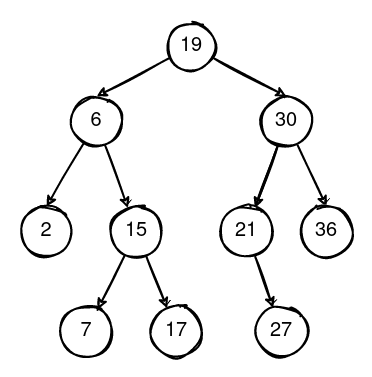
\includegraphics[width=.45\linewidth]{images/abb1}
\end{center}


\end{frame}


\begin{frame}[fragile]
 \frametitle{ABB: Árbol binario de búsqueda}
\small
En un árbol binario de búsqueda, los hijos izquierdos guardan información menor (o igual), y los hijos derechos guardan información mayor, con respecto a la de su padre.

\begin{center}
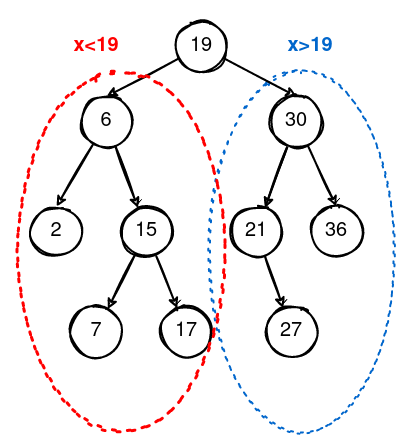
\includegraphics[width=.45\linewidth]{images/abb2}
\end{center}
\end{frame}

\begin{frame}[fragile]
 \frametitle{ABB: Árbol binario de búsqueda}
\small
\begin{center}
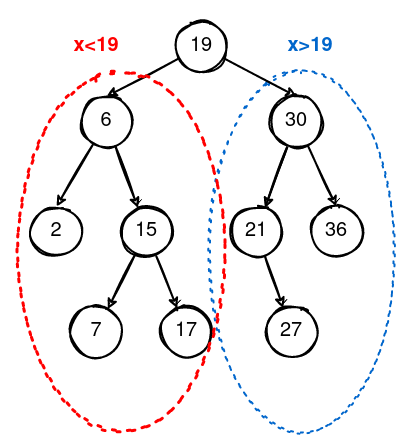
\includegraphics[width=.45\linewidth]{images/abb2}
\end{center}

A partir de esta regla de modelamiento se definen fácilmente las operaciones de búsqueda, inserción, y eliminación de elementos. Además de que los recorridos pre-orden, in-orden y post-orden sean efectivos para determinadas labores.
\end{frame}



\begin{frame}[fragile]
 \frametitle{ABB: Árbol binario de búsqueda}
\small
Por ejemplo, es fácil determinar el lugar y posición de los valores en un intervalo. 

\begin{center}
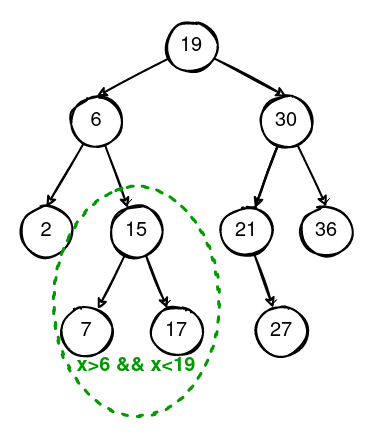
\includegraphics[width=.35\linewidth]{images/abb3}
\end{center}

\begin{itemize}
\item \textbf{¿Cómo determinan el sucesor y predecesor de un padre?}\\
{\color{red}{Sucesor: buscar en la derecha, todo hacia la izquierda.}}\\
{\color{blue}{Antecesor: buscar en la izquierda, todo hacia la derecha.}} \\
\item \textbf{¿Cuál es su principal característica?}\\
{\color{red}{Siempre tendrán a lo más un hijo.}}
\end{itemize}
\end{frame}


\begin{frame}[fragile]
 \frametitle{ABB: Operaciones}
\small Las operaciones más comunes de los ABB son:

\begin{itemize}
\item \texttt{init()}: Inicializar el árbol (root == NULL).
\item \texttt{size()}: Cantidad de elementos en el árbol.
\item \texttt{x\_preorden()}: Operación x en pre-orden.
\item \texttt{x\_inorden()}: Operación x en in-orden. 
\item \texttt{x\_postorden()}: Operación x en post-orden. 
\item \texttt{search()}: Buscar un elemento en el árbol.
\item \texttt{insert()}: Insertar un elemento en el árbol.
\item \texttt{delete()}: Eliminar un elemento en el árbol.
\item \texttt{clear()}: Limpiar el árbol.
\end{itemize}
\end{frame}

\begin{frame}[fragile]
 \frametitle{ABB: Recorrer}
\small
¿Como se imprimirían los datos del siguiente árbol con recorrido pre-orden, in-orden y post-orden?

\begin{center}
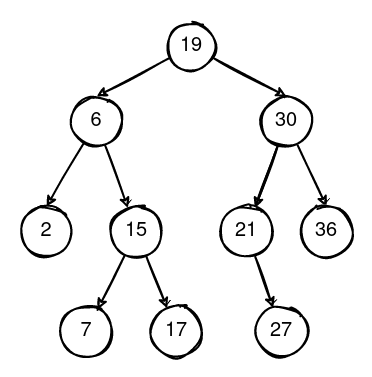
\includegraphics[width=.45\linewidth]{images/abb1}
\end{center}

\pause
\begin{itemize}
\item Pre-orden: 19 - 6 - 2 - 15 - 7 - 17 - 30 - 21 - 27 - 36 \pause
\item In-orden: 2 - 6 - 7 - 15 - 17 - 19 - 21 - 27 - 30 - 36 \pause
\item Post-orden: 2 - 7 - 17 - 15 - 6 - 27 - 21 - 36 - 30 - 19 
\end{itemize}


\end{frame}


\begin{frame}[fragile]
 \frametitle{ABB: Buscar}
Comenzaremos con la función básica \texttt{search()}: Buscar un elemento en el árbol.

\begin{center}
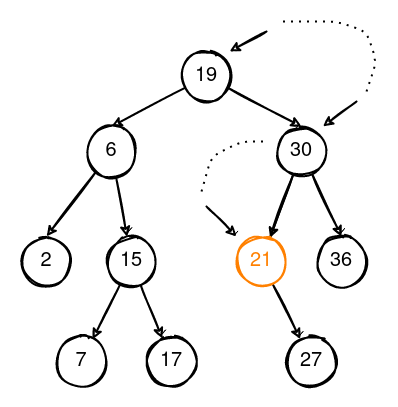
\includegraphics[width=.35\linewidth]{images/abb-search}
\end{center}

Se puede hacer de dos formas:
\begin{itemize}
\item Usando un puntero para recorrer el árbol.
\item \textbf{Recursivamente}.
\end{itemize}
\end{frame}

\begin{frame}[fragile]
 \frametitle{ABB: Buscar}

\begin{exampleblock}{Recursivamente}
\begin{lstlisting}[language=C, basicstyle=\tiny, escapeinside={\\}{\\}]
int * search(nodo_t * raiz, int value){ 

	if(raiz == NULL || raiz->dato == value) //{} omitidas
		return raiz;
	else if(value < raiz->dato)
		return search(raiz->hijo_izq, value);
	else if(value > raiz->dato) // else
		return search(raiz->hijo_der, value);
	
}
\end{lstlisting}
\end{exampleblock}

\begin{block}{Usando Puntero}
\begin{lstlisting}[language=C, basicstyle=\tiny, escapeinside={|}{|}]
int * search(nodo_t * raiz, int value){
	
	nodo_t * rec = raiz;
	while(rec!=NULL){
		if(rec->dato == value){
			return rec;
		}else if(value < rec->dato){
			rec = rec->hijo_izq;
		}else if(value > rec->dato){
			rec = rec->hijo_der;
		}
	return rec; // NULL si no lo encuentra o arbol vacío
}
\end{lstlisting}
\end{block}


\end{frame}

\begin{frame}[fragile]
 \frametitle{ABB: Insertar}
\small
Para poder insertar debemos buscar primero el lugar donde debe realizarse la inserción. La idea es \textbf{mantener} el orden de nuestro ABB.

\begin{center}
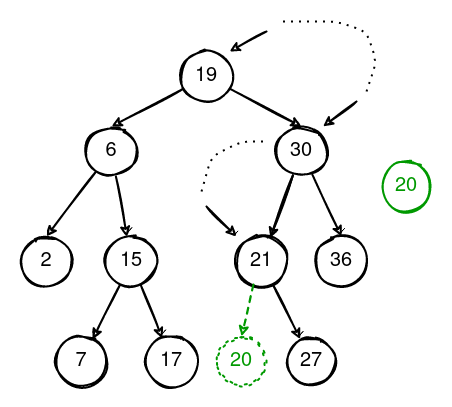
\includegraphics[width=.45\linewidth]{images/abb-insert}
\end{center}

Nota: Si nuestro árbol no acepta elementos repetidos, al encontrar el valor se detiene.

\end{frame}

\begin{frame}[fragile]
 \frametitle{ABB: Insertar}
\begin{exampleblock}{Recursivamente}
\begin{lstlisting}[language=C, basicstyle=\tiny, escapeinside={|}{|}]
void insert(nodo_t ** raiz, int value){ 

	if(*raiz == NULL){
		*raiz = malloc(sizeof(node_t));
		(*raiz)-> dato = value;
		(*raiz)->hijo_izq = NULL;
		(*raiz)->hijo_der = NULL;

	}else if(value < (*raiz)->dato){
		insert(&((*raiz)->hijo_izq), value);

	}else if(value > (*raiz)->dato){
		insert(&((*raiz)->hijo_der), value);
	}
}
\end{lstlisting}
\end{exampleblock}
\end{frame}

\begin{frame}[fragile]
 \frametitle{ABB: Insertar}
Cree el árbol binario que represente la siguiente secuencia de enteros: 
$$ 10 - 5 - 7 - 14 - 12 - 18 - 15 $$\pause
\begin{alertblock}{Spoiler}
\begin{center}
\visible<.(1)>{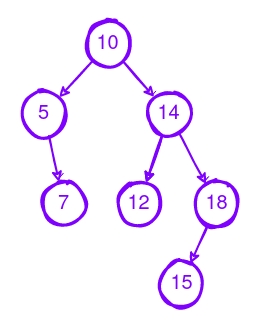
\includegraphics[width=.35\linewidth]{images/abb-insert-example}}
\end{center}
\end{alertblock}
\end{frame}

\begin{frame}[fragile]
 \frametitle{ABB: Eliminar}
\small
Al igual que en insertar, deberemos buscar el nodo a eliminar. Pero para poder eliminarlo, tendremos que considerar los siguientes casos:

\begin{itemize}
\item Nodo objetivo es una hoja (no tiene hijos).
\item Nodo objetivo tiene un sólo hijo.
\item Nodo objetivo tiene dos hijos.
\end{itemize}

\end{frame}

\begin{frame}[fragile]
 \frametitle{ABB: Eliminar hoja.}
\small
Es el caso más sencillo, solo corresponde a liberar el nodo desde el puntero del padre.

\begin{center}
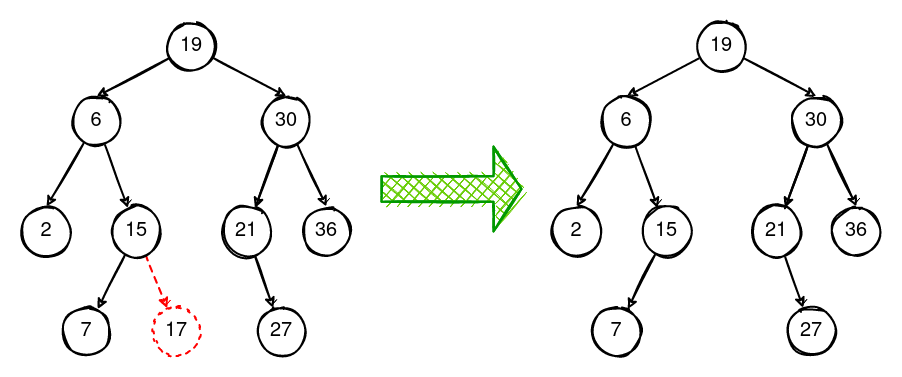
\includegraphics[width=.9\linewidth]{images/abb-delete-nochild}
\end{center}
\end{frame}

\begin{frame}[fragile]
 \frametitle{ABB: Eliminar nodo con 1 hijo.}
\small
Caso intermedio. acá se elimina el nodo encontrado, pero su posición es ocupada por su único hijo. Se eleva ese sub-árbol, un nivel.

\begin{center}
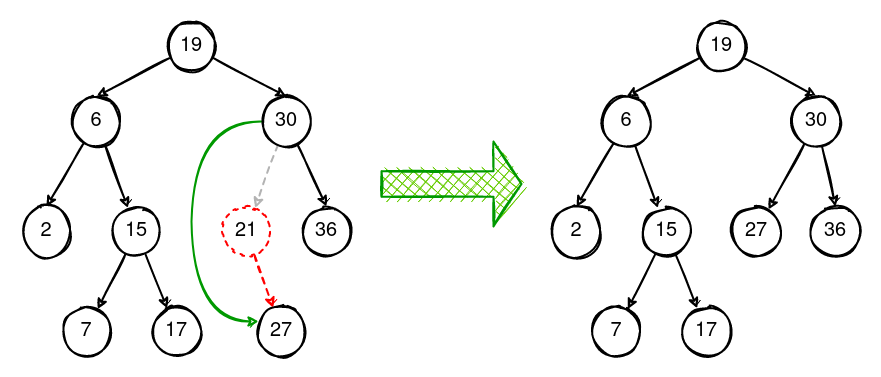
\includegraphics[width=.9\linewidth]{images/abb-delete-onechild}
\end{center}
\end{frame}

\begin{frame}[fragile]
 \frametitle{ABB: Eliminar nodo con 2 hijos.}
\small
Caso recursivo o iterativo. Cuenta de dos pasos:
\begin{itemize}
\item Reemplazar el nodo objetivo por una copia de su sucesor o antecesor (uds. eligen).
\item Borrar el sucesor o antecesor original.
\end{itemize}

\begin{center}
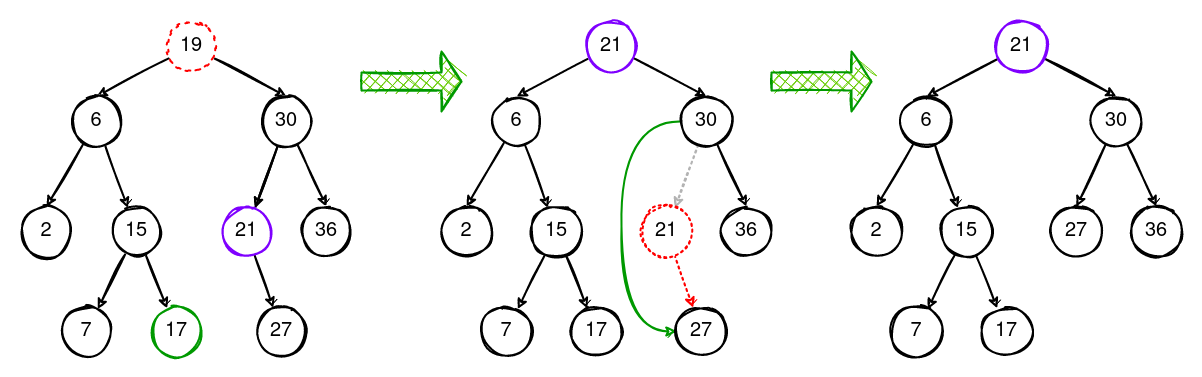
\includegraphics[width=\linewidth]{images/abb-delete-twochild}
\end{center}
\end{frame}



\begin{frame}[fragile]
 \frametitle{ABB: Insertar}
\begin{exampleblock}{Recursivamente}
\begin{lstlisting}[language=C, basicstyle=\tiny, escapeinside={|}{|}]
int delete(nodo_t ** raiz, int value){ 
	// ¿Cómo lo programan?
	// Necesitarán alguna función extra.
}
\end{lstlisting}
\end{exampleblock}
\end{frame}

\begin{frame}[fragile]
 \frametitle{Ejercicios}
\begin{itemize}
\item Para el siguiente conjunto $\{1, 4, 5, 10, 16, 17, 21\}$, dibuje árboles binarios de búsqueda con altura 2, 3, 4, 5, y 6.
\item Escriba funciones recursivas para recorrer un árbol binario de búsqueda en pre-orden y post-orden.
\item Asuma que tiene números entre 1 y 1000 en un árbol binario de búsqueda y quiere buscar el nodo 363. ¿Cuál de las siguientes secuencias de nodos NO podría ser una secuencia de nodos examinados en el árbol para llegar al nodo 363?
\begin{enumerate}
\item 2, 252, 401, 398, 330, 344, 397, 363.
\item 924, 220, 911, 244, 898, 258, 362, 363.
\item 925, 202, 911, 240, 912, 245, 363.
\item 2, 399, 387, 219, 266, 382, 381, 278, 363.
\item 935, 278, 347, 621, 299, 392, 358, 363.
\end{enumerate}
\end{itemize}
\end{frame}

%\section{Recursividad}
%%funciones recursivas
%
%\begin{frame}[fragile]
% \frametitle{Recursividad}
%
%Los procesos recursivos son aquellos ciclos autorreferentes, vale decir, una definición (matemática, funciones, programas) depende parcialmente de sí misma. 
%
%\begin{center}
%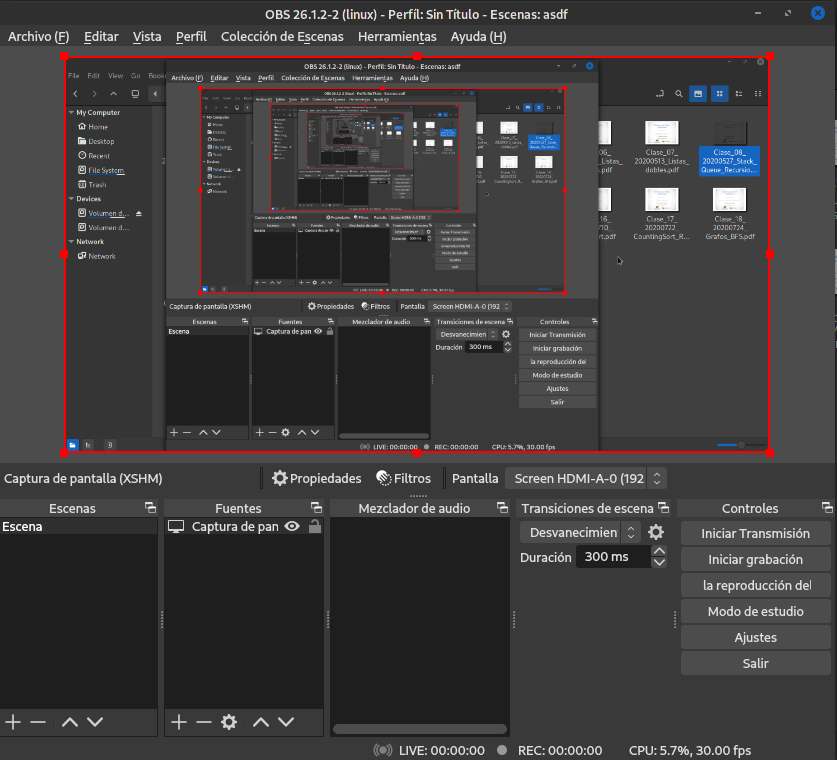
\includegraphics[width=.7\linewidth]{images/obs-recursion}
%\end{center}
%
%\end{frame}
%
%\begin{frame}[fragile]
% \frametitle{Recursividad}
%Una definición recursiva se compone de dos elementos básicos:
%\begin{enumerate}
%\item Un caso base que detiene el ciclo.
%\item Una llamada autorreferente con un elemento. 
%\end{enumerate}
%
%\begin{block}{Factorial}
%$ f(0) = 1 $\\
%$ f(n) = n \times f(n-1)$.
%\end{block}
%
%\begin{exampleblock}{Factorial en C}
%\begin{lstlisting}[language=C, basicstyle=\tiny, escapeinside={|}{|}]
%int factorial(int n){
%	if (n<0)
%		return -1; //Valor de Error
%	elif(n==0) // caso base, sin condicion -> loop infinito
%		return 1; 
%	return n * factorial(n-1); // llamado a un elemento parcial del caso
%}
%
%\end{lstlisting}
%\end{exampleblock}
%Entenderemos por recursivdad como la técnica en la cual alguna función depende de su propia definición, vale decir, \textbf{se llama a sí misma} para formar un ciclo.
%\end{frame}
%
%\begin{frame}[fragile]
% \frametitle{Recursividad: Ejemplos}
%\begin{enumerate}
%\item Sequencia de Fibonacci.
%\item Polinomio de Hermite.
%\item Triángulo de Pascal.
%\item Fractales.
%\begin{itemize}
%\item Curva de Peano.
%\item Curva de Koch.
%\item Curva de Hilbert. 
%\end{itemize}
%\item \textbf{Árboles}.
%\end{enumerate}
%\end{frame}
%
%
%\section{Árboles}
%%conceptos de árboles, recursivadad en teoria
%\begin{frame}[fragile]
% \frametitle{Árboles}
%
%Los árboles son una estructura de dato no-lineal, jerárquica y enlazada que permite acceso eficiente a los elementos de la estructura tanto como a actualización de la misma.
%
%\begin{center}
%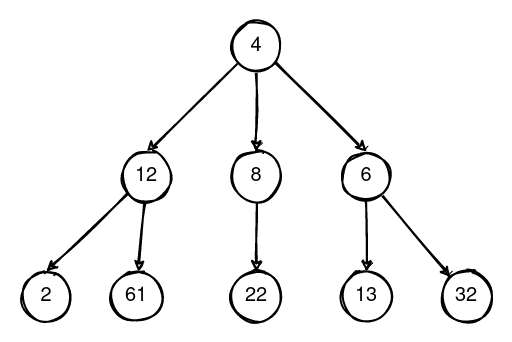
\includegraphics[width=.7\linewidth]{images/arbol1}
%\end{center}
%
%\end{frame}
%
%\begin{frame}[fragile]
% \frametitle{Árboles: Aplicaciones}
%Los árboles son extensamente utilizados en diversas áreas de las telecomunicaciónes, tecnologías de la información, matemáticas, electrónica e informática:
%\begin{itemize}
%\item Compilación e interpretación de elementos sintácticos de un lenguaje.
%\item Representación expresiones aritméticas y/o lógicas.
%\item Representación de estructuras de búsqueda de datos.
%\item Sistemas de archivos y directorios.
%\item Clases y herencia en POO.
%\item Compresión de datos
%\item Computación Evolutiva.
%\end{itemize}
%\end{frame}
%
%\begin{frame}[fragile]
% \frametitle{Árboles: Conceptos}
%
%Un árbol está formado por un conjunto finito de elementos, llamados nodos los cuales son enlazados entre sí según jerarquía padre-hijo.
%\begin{itemize}
%\item Primer nodo $\rightarrow$  raíz del árbol.
%\item Relación padre-hijo $\rightarrow$ jerarquía.
%\item Nodos $\rightarrow$ varios sucesores.
%\item Nodos $\rightarrow$ único antecesor.
%\end{itemize}
%
%\begin{center}
%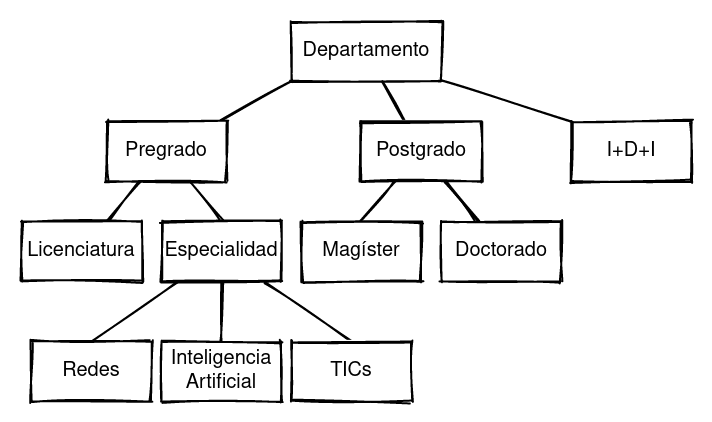
\includegraphics[width=.6\linewidth]{images/example1}
%\end{center}
%
%\end{frame}
%
%\begin{frame}[fragile]
% \frametitle{Árboles: Conceptos}
%\small
%Los componentes de los árboles son nombrados y clasificados según sus características.
%\begin{itemize}
%\item Primer nodo $\rightarrow$  raíz del árbol.
%\item Nodo con sucesores $\rightarrow$ padre.
%\item Sucesor de un nodo $\rightarrow$ hijo.
%\item Nodos con padre e hijos $\rightarrow$ nodo intermedio.
%\item Nodo sin hijos $\rightarrow$ hoja (nodo terminal).
%\end{itemize}
%
%\begin{center}
%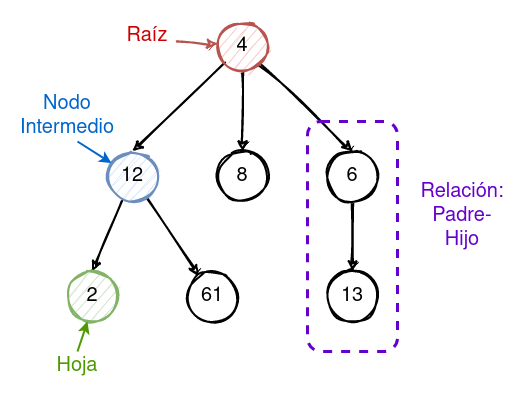
\includegraphics[width=.6\linewidth]{images/concepto}
%\end{center}
%
%\end{frame}
%
%\begin{frame}[fragile]
% \frametitle{Árboles: Conceptos}
%\small
%Además en un árbol, se identifica la siguiente información:
%\begin{itemize}
%\item Camino: Secuencia entre dos nodos siguiendo relación jerárquica padre hijo.
%$$\text{camino}(4,47)=\{4,12,61,47\}$$ 
%\item Largo Camino: Número de enlaces (nodos-1) entre dos nodos en relación jerárquica.
%$$\text{largo}(4,47)=3$$ 
%\item Rama: Camino de la raíz a una hoja.
%$$\text{rama}_1 = \text{camino}(4,2)$$
%\end{itemize}
%
%\begin{center}
%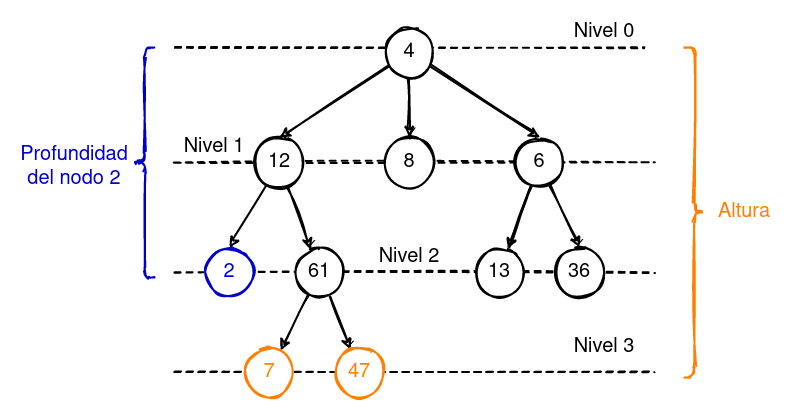
\includegraphics[width=.67\linewidth]{images/concepto2}
%\end{center}
%\end{frame}
%
%\begin{frame}[fragile]
% \frametitle{Árboles: Conceptos}
%\small
%\begin{itemize}
%\item Grado de Nodo: Cantidad de hijos.
%$$\text{grado}(47)=0$$ 
%\item Grado del árbol: Máximo número de hijos para cada nodo.
%$$\text{grado}(A)=3$$ 
%\item Profundidad: Cantidad de predecesores del nodo.
%$$\text{profundidad}(2) = 2$$
%\end{itemize}
%
%\begin{center}
%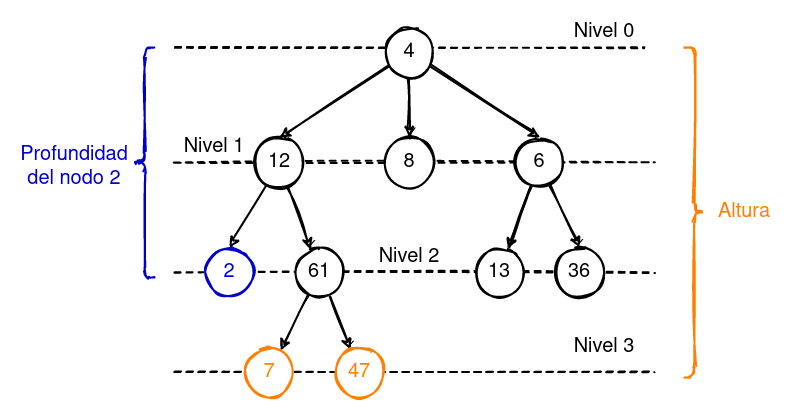
\includegraphics[width=.67\linewidth]{images/concepto2}
%\end{center}
%
%\end{frame}
%
%\begin{frame}[fragile]
% \frametitle{Árboles: Conceptos}
%\small
%\begin{itemize}
%\item Altura: Profundidad Máxima de los nodos o largo del camino más grande. 
%$$\text{altura}(A)=3$$ 
%\item Nivel: Número de enlaces del camino de la raíz al nodo (parte en 0). 
%$$\text{nivel}(4)=3$$ 
%\item Bosque: Colección o conjunto de árboles.
%\end{itemize}
%
%\begin{center}
%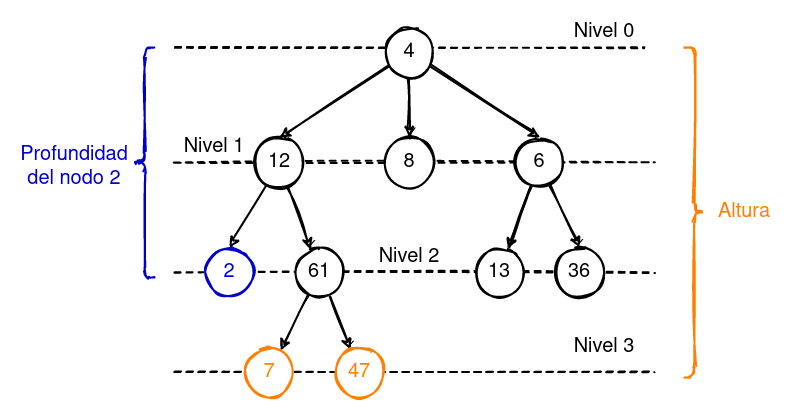
\includegraphics[width=.67\linewidth]{images/concepto2}
%\end{center}
%
%\end{frame}
%
%\begin{frame}[fragile]
% \frametitle{Árboles: Recursividad}
%\small
%Los árboles son estructuras de datos recursiva, debido a que cada hijo de un nodo es la raíz de un árbol de menor altura (sub-árbol). 
%
%
%\begin{center}
%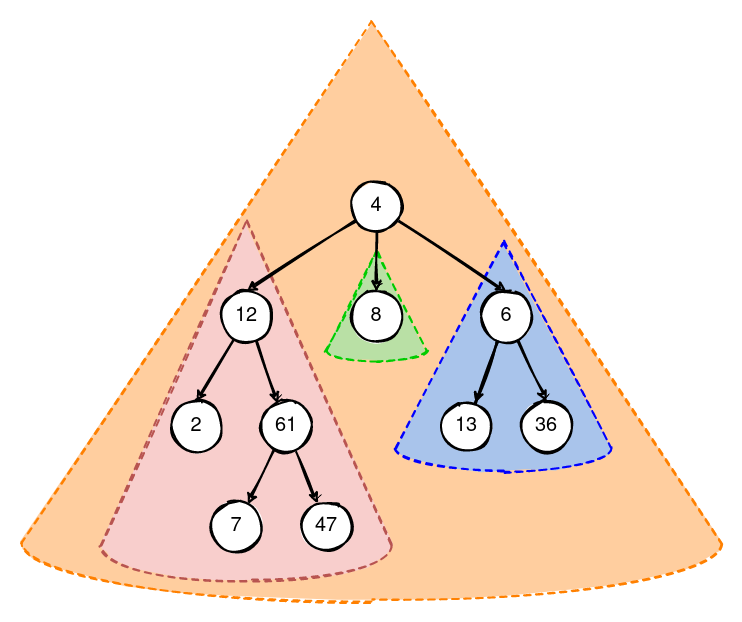
\includegraphics[width=.6\linewidth]{images/arbolrecursivo}
%\end{center}
%
%
%Por esta razón. las funciones y métodos de árboles son facilmente aplicables con técnicas recursivas.
%\end{frame}
%
%\section{Árboles Binarios}
%\begin{frame}[fragile]
% \frametitle{Árboles binarios}
%\small
%En este curso nos concentraremos en árboles binarios, i.e., árboles cuyo grado es 2. 
%
%\begin{center}
%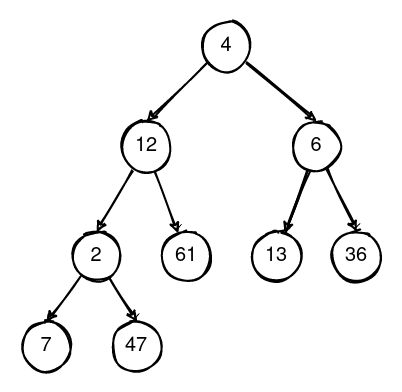
\includegraphics[width=.4\linewidth]{images/binarytree}
%\end{center}
%
%Aplicaciones:
%\begin{itemize}
%\item Gramática de lenguajes, i.e. matemáticas.
%\item Árboles de Decisión.
%\item \textbf{Árbol Binario de Búsqueda.}
%\end{itemize}
%
%\end{frame}
%
%\begin{frame}[fragile]
% \frametitle{Árboles binarios: Implementación}
%\small
%Un árbol binario tiene a lo más dos hijos, y se implementa muy similar a las listas enlazadas.
%
%\begin{center}
%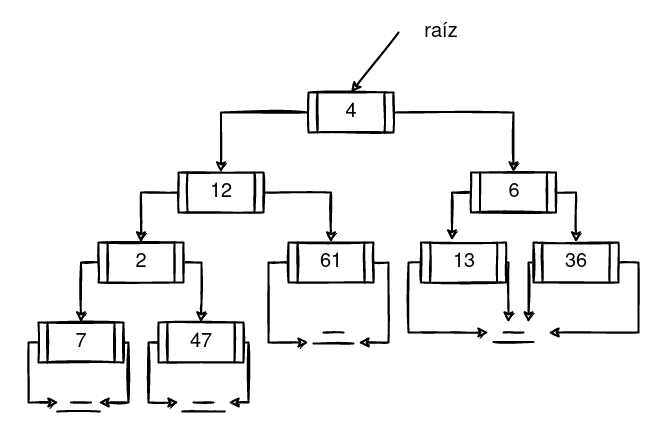
\includegraphics[width=.55\linewidth]{images/binarytree2}
%\end{center}
%
%\begin{exampleblock}{Árbol Binario en C}
%\begin{lstlisting}[language=C, basicstyle=\tiny, escapeinside={|}{|}]
%typedef struct nodo{
%	int dato;
%	struct nodo *hijo_izq;
%	struct nodo *hijo_der;
%} nodo_t;
%
%int main(int argc, char **argv){
%	nodo_t *raiz; // árbol vacío
%	return 0;
%}
%
%\end{lstlisting}
%\end{exampleblock}
%\end{frame}
%
%\begin{frame}[fragile]
% \frametitle{Árboles binarios: Implementación}
%\small
%
%\begin{center}
%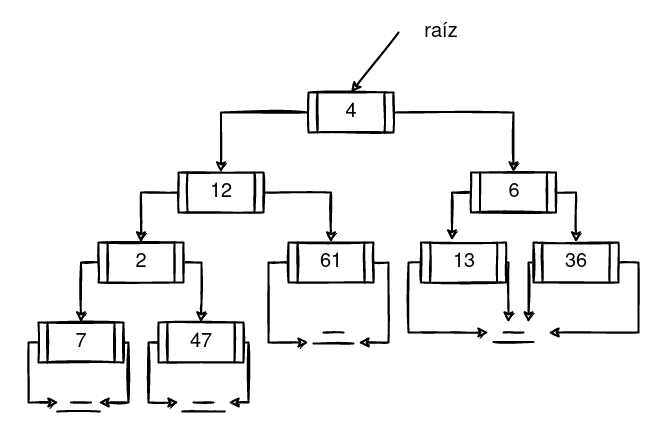
\includegraphics[width=.7\linewidth]{images/binarytree2}
%\end{center}
%
%Detalles:
%\begin{itemize}
%\item El puntero de control se encuentra siempre en la raíz. 
%\item Los nodos cuyos hijos apunten a \texttt{NULL}, son hojas.
%\item \textbf{¿Cómo podemos recorrer un árbol (binario)?.} - En seguida.
%\item \textbf{¿Cómo agregar, buscar, eliminar elementos de un árbol binario?} - ABB: Próxima clase.
%\end{itemize}
%\end{frame}
%
%
%\begin{frame}[fragile]
% \frametitle{Árboles binarios: Recorridos}
%\small 
%Muchas aplicaciones necesitan procesar un árbol visitando sus nodos, y realizando acciones sobre ellos: \textit{mostrar su contenido}, \textit{sumar valores guardados}, \textit{encontrar un nodo específico}, etc.\\
%\bigskip
%Explicaremos dos de las formas más clásicas para recorrer un árbol:
%\begin{itemize}
%\item Recorrido en anchura.
%\item Recorrido en profundidad.
%\end{itemize}
%\end{frame}
%
%
%\begin{frame}[fragile]
% \frametitle{Árboles binarios: Recorrido en Anchura}
%\small 
%Tiene como criterio visitar todos los nodos de un nivel antes de pasar al siguiente.
%
%\begin{center}
%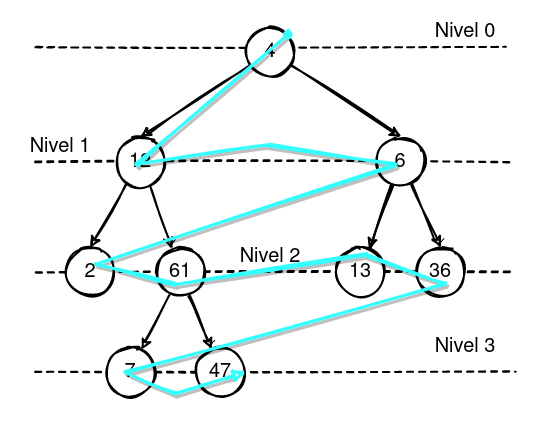
\includegraphics[width=.55\linewidth]{images/breadthsearch}
%\end{center}
%
%
%\begin{itemize}
%\item No puede realizarse directamente por recursividad.
%\item Se utiliza una \textbf{Queue/Cola} como estructura auxiliar.
%\item Recorre todos los nodos de un nivel, antes de pasar al siguiente. 
%\item Se realiza dequeue y enqueues hasta pasar por todos lo niveles.
%\end{itemize}
%
%\end{frame}
%
%
%\begin{frame}[fragile]
% \frametitle{Árboles binarios: Recorrido en Profundidad}
%\small 
%Tiene como criterio visitar los nodos por profundidad hasta llegar una hoja, luego retrocede y continúa.
%\begin{center}
%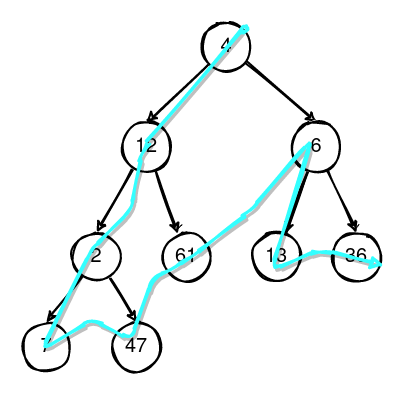
\includegraphics[width=.45\linewidth]{images/dfs1}
%\end{center}
%
%Tres de los tipos de recorrido en profundidad más utilizados son:
%\begin{itemize}
%\item Pre-orden.
%\item In-orden.
%\item Post-orden.
%\end{itemize}
%
%\end{frame}
%
%\begin{frame}[fragile]
% \frametitle{Árboles binarios: Rec. Prof. Pre-orden}
%\small 
%Recorrido recursivo que sigue la siguiente orden de visitas:
%\begin{enumerate}
%\item Visitar nodo actual.
%\item Visitar hijo izquierdo en pre-orden.
%\item Visitar hijo derecho en pre-orden.
%\end{enumerate}
%
%\begin{center}
%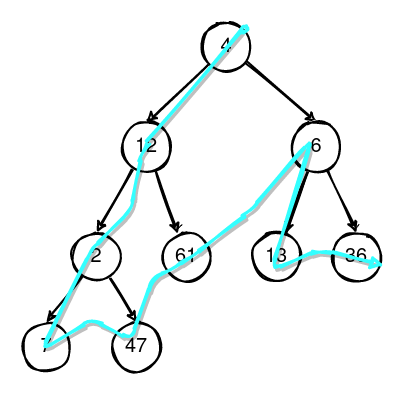
\includegraphics[width=.4\linewidth]{images/dfs1}
%\end{center}
%\end{frame}
%
%\begin{frame}[fragile]
% \frametitle{Árboles binarios: Rec. Prof. Pre-orden}
%\small 
%
%\begin{center}
%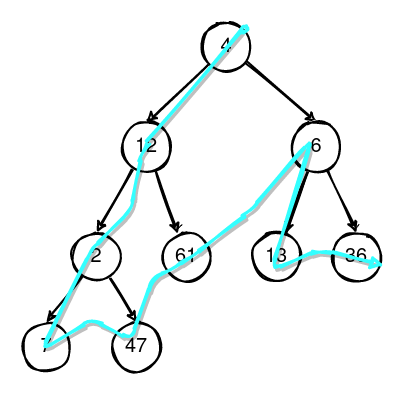
\includegraphics[width=.4\linewidth]{images/dfs1}
%\end{center}
%
%\begin{exampleblock}{Pre-orden en C}
%\begin{lstlisting}[language=C, basicstyle=\tiny, escapeinside={|}{|}]
%void print_preorden(node_t *root){
%	printf("Dato: |\%|d\n", root->dato);
%	
%	if(root->hijo_izq != NULL)
%		print_preorden(root->hijo_izq);
%
%	if(root->hijo_der != NULL)
%		print_preorden(root->hijo_der);
%}
%\end{lstlisting}
%\end{exampleblock}
%\end{frame}
%
%
%
%
%\begin{frame}[fragile]
% \frametitle{Árboles binarios: Rec. Prof. In-orden}
%\small 
%Recorrido recursivo que sigue la siguiente orden de visitas:
%\begin{enumerate}
%\item Visitar hijo izquierdo en in-orden.
%\item Visitar nodo actual.
%\item Visitar hijo derecho en in-orden.
%\end{enumerate}
%
%\begin{center}
%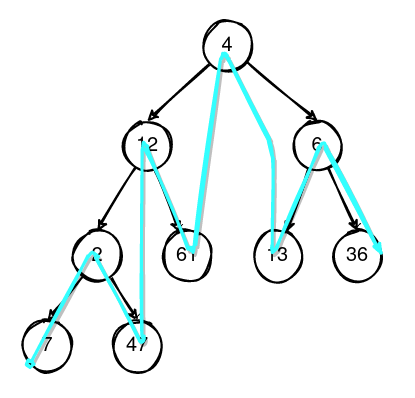
\includegraphics[width=.4\linewidth]{images/dfs2}
%\end{center}
%\end{frame}
%
%\begin{frame}[fragile]
% \frametitle{Árboles binarios: Rec. Prof. In-orden}
%\small 
%
%\begin{center}
%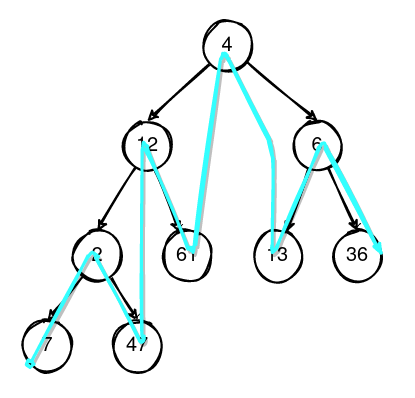
\includegraphics[width=.4\linewidth]{images/dfs2}
%\end{center}
%
%\begin{exampleblock}{In-orden en C}
%\begin{lstlisting}[language=C, basicstyle=\tiny, escapeinside={|}{|}]
%void print_inorden(node_t *root){
%
%	if(root->hijo_izq != NULL)
%		print_inorden(root->hijo_izq);
%
%	printf("Dato: |\%|d\n", root->dato);
%	
%
%	if(root->hijo_der != NULL)
%		print_inorden(root->hijo_der);
%}
%\end{lstlisting}
%\end{exampleblock}
%\end{frame}
%
%
%
%\begin{frame}[fragile]
% \frametitle{Árboles binarios: Rec. Prof. Post-orden}
%\small 
%Recorrido recursivo que sigue la siguiente orden de visitas:
%\begin{enumerate}
%\item Visitar hijo izquierdo en post-orden.
%\item Visitar hijo derecho en post-orden.
%\item Visitar nodo actual.
%\end{enumerate}
%
%\begin{center}
%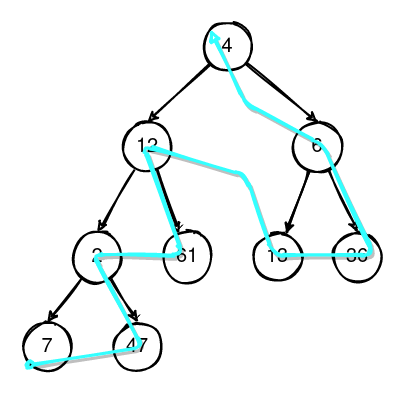
\includegraphics[width=.4\linewidth]{images/dfs3}
%\end{center}
%\end{frame}
%
%\begin{frame}[fragile]
% \frametitle{Árboles binarios: Rec. Prof. Post-orden}
%\small 
%
%\begin{center}
%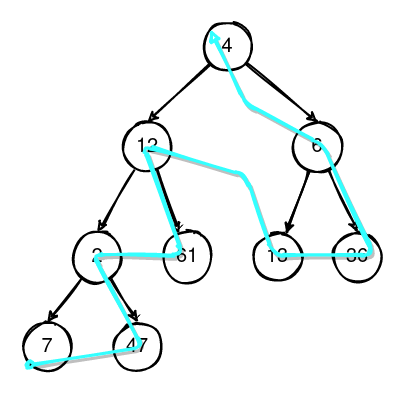
\includegraphics[width=.4\linewidth]{images/dfs3}
%\end{center}
%
%\begin{exampleblock}{Post-orden en C}
%\begin{lstlisting}[language=C, basicstyle=\tiny, escapeinside={|}{|}]
%void print_postorden(node_t *root){
%
%	if(root->hijo_izq != NULL)
%		print_postorden(root->hijo_izq);
%
%	if(root->hijo_der != NULL)
%		print_postorden(root->hijo_der);
%
%	printf("Dato: |\%|d\n", root->dato);
%}
%\end{lstlisting}
%\end{exampleblock}
%\end{frame}


%conceptos de árboles binarios y búsqueda en profundidad. recursivdad en teoria


%\section{Árbol Binario Busqueda}
%regla menor a la izq, mayor a la derecha
%implementar recorrer: 3 metodos.
%metdos, insertar, buscar, elimnar -> modificar (combination).
%recursividad en practica


%\begin{frame}[fragile]
% \frametitle{Lista Simple Enlazada: Inicializar}
%
%Las listas, en su versión más básica, dependen de un puntero al inicio de la lista. Éste suele llamarse \textit{header}, \textit{cabecera} o  \textit{inicio}.
%\begin{exampleblock}{C}
%\begin{lstlisting}[language=C, basicstyle=\tiny, escapeinside={|}{|}]
%#include<stdio.h>
%
%typedef struct nodo{
%	int dato; //dato, puede ser lo que uds. necesiten
%	struct nodo *sgte; // puntero a un nodo enalce.
%} nodo_t;
%
%int main(int argc, char **argv){
%
%	nodo_t * inicio = NULL; 
%	// Inicializamos la lista, con su puntero de inicio apuntando a NULL
%	// Equivalente a lista vacía []
%
%	return 0;
%}
%\end{lstlisting}
%\end{exampleblock}
%\end{frame}
%
%\begin{frame}[fragile]
% \frametitle{Lista Simple Enlazada: Inicializar}
%\begin{center}
%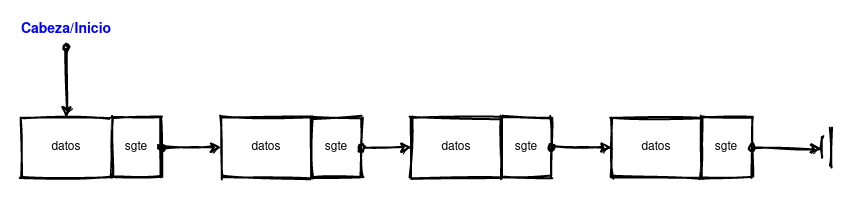
\includegraphics[width=.9\linewidth]{images/linkedlist1}
%\end{center}
%
%\end{frame}



\end{document}
